\chapter{Background} \label{chap1}
In 2015, an epoch when LIGO detectors have detected gravitational-waves (GW), new astronomy had been established. From the first detection, the development of GW detectors has been a history of improving sensitivity. It is necessary to improve the duty cycle, which is the observable time, as well as the sensitivity because the GW astronomy needs multiple detectors to determine the direction of the arrival. 

This chapter describes GW and GW detectors. GWs cause strain changes in space which are extremely small. In order to detect the strain, the GW detector is a complex Michelson interferometer with several optical resonators. In addition, in order to increase the sensitivity of strain measurement, the baseline is enlarged. The complicated and large interferometer has a limited duty cycle due to seismic noise. This chapter focuses on the duty cycle of the terrestrial large-scale GW detector because the purpose of this thesis is the development of the new seismic isolation system to improve the duty cycle.

In section \cref{sec:11}, we describe the essential properties and sources of the gravitational-wave. Section \cref{sec:12} describes the detection principle of the GW by using an interferometer. In section \cref{sec:13} and \cref{sec:14}, we describe the technology to improve the sensitivity of the detectors and the duty cycle of the current terrestrial detectors, respectively. At the end of the chapter, we describe the outline of this thesis in section \cref{sec:15}.

\section{Gravitational-wave (GW)} \label{sec:11}
Gravitational-wave (GW) is a ripple of the space-time which propagates at the speed of light. These waves are generated by the dynamic motion of the massive object in the universe. Therefore, the GW informs us not only the feature of the space-time but also the mechanism of the high-energy astrophysical phenomena.

\subsection{Properties of GWs}
GW was predicted by A. Einstein in 1918 and is a result of the general theory of relativity. 

\subsubsection{Two polarized transverse waves}
The metric tensor $g_{\mu\nu}$ describes the interval between two events in space-time as, 
\begin{eqnarray}
  d s^{2}=g_{\mu \nu} d x^{\mu} d x^{\nu} (\mu,\nu = 0,1,2,3),
\end{eqnarray}
where $dx^{\mu}$ represents the coordinate distance of the events, and $x^{\mu}$ has four components; $(ct,x,y,z)$.

In the general relativity theory \cite{einstein1916vd}, the metric tensor $g_{\mu\nu}$ is described by Einstein's equation;
\begin{eqnarray}
  R_{\mu \nu}\left(g_{\mu \nu}\right)-\frac{1}{2} g_{\mu \nu} R\left(g_{\mu \nu}\right)=\frac{8 \pi G}{c^{4}} T_{\mu \nu},
\end{eqnarray}
where $R_{\mu\nu}$ is the Ricci tensor, $R=g^{\mu \nu} R_{\mu \nu}$ is the Ricci scalar curvature, $T_{\mu\nu}$ is the energy-momentum tensor, $G$ is Newton's gravitational constant, and $c$ is the speed of light.

\begin{figure}[t]
  \begin{center}   
    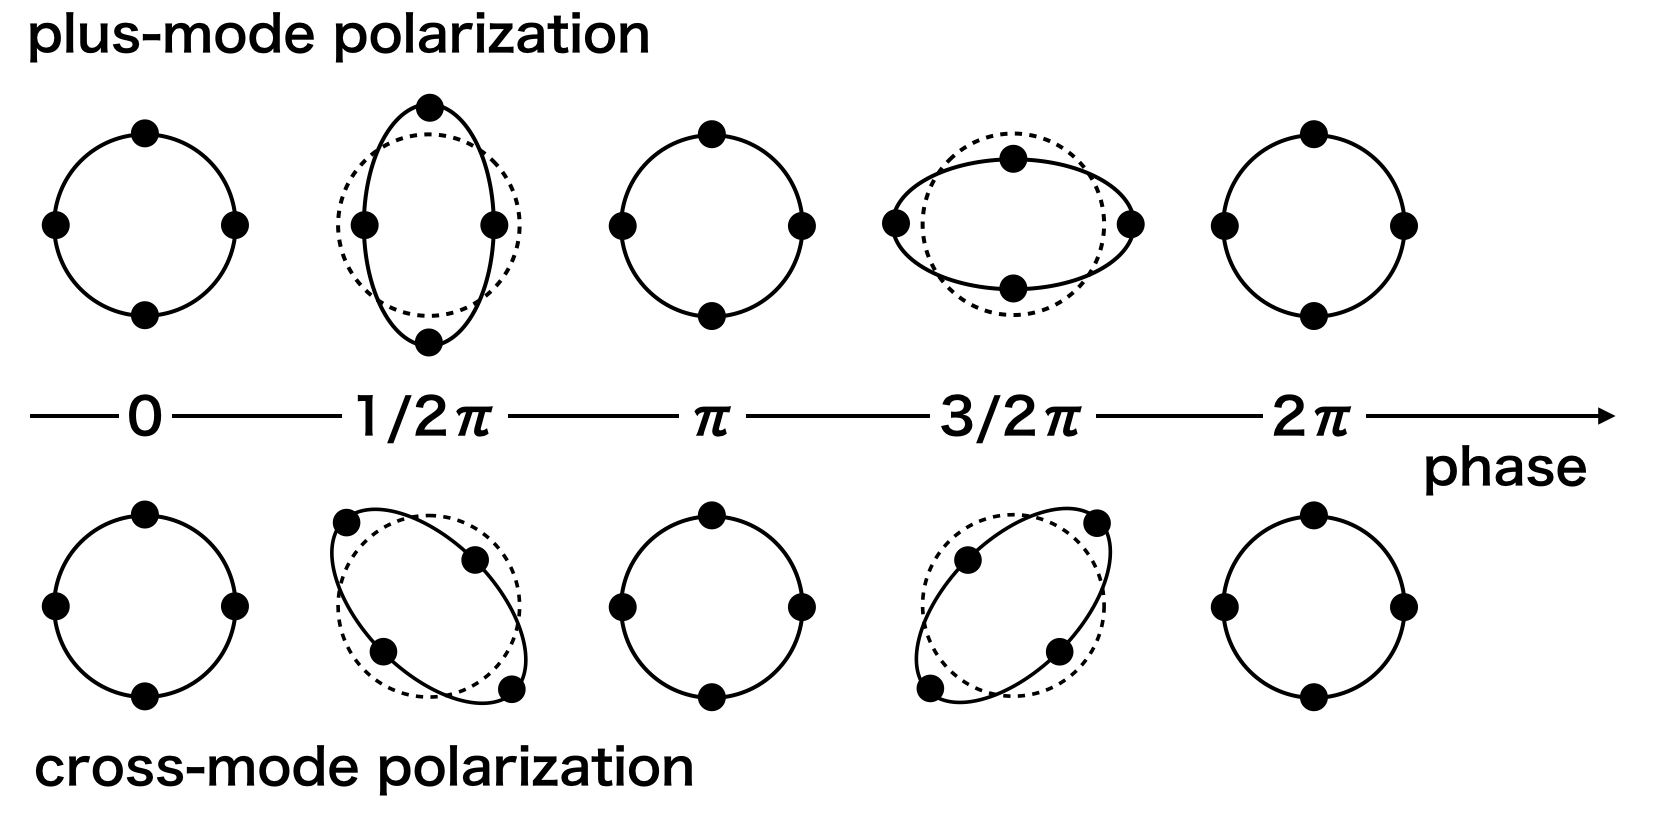
\includegraphics[width=11.0cm]{./img_chap1/img131.png}
    \caption{Polarizations of the GW propagating in the direction of the paper. These polarizations change the distance as the tidal motion. }\label{img:img131}
  \end{center}
\end{figure}

GW is derived from Einstein's equation when the metric can be described as the perturbation to the metric $h_{\mu\nu}$ and the Minkowsky metric describing flat space-time $\eta_{\mu\nu}$, thus
\begin{eqnarray}
  g_{\mu \nu}\sim\eta_{\mu \nu}+h_{\mu \nu}.
\end{eqnarray}
In this weak-field regime, Einstein's equation reduces a linearized wave-equation whose solution is represented as
\begin{eqnarray}
  h_{\mu \nu}(z, t)=\left(\begin{array}{cccc}{0} & {0} & {0} & {0} \\ {0} & {-h_{+}} & {h_{\times}} & {0} \\ {0} & {h_{\times}} & {h_{+}} & {0} \\ {0} & {0} & {0} & {0}\end{array}\right) \cos \left[\omega\left(\mathrm{t}-\frac{\mathrm{Z}}{\mathrm{c}}\right)\right], \label{eq:eq130}
\end{eqnarray}
where $\omega$ is the angular frequency of GW, z is the propagation direction of the wave, $h_{+}$ and $h_{\times}$ are the independent polarization of that. Therefore, GW is the transverse wave propagating with the speed of light.

The two polarizations of GW are known as plus and cross polarizations, and these polarizations change the distance between two points, as shown in Figure \ref{img:img131}. 


\subsection{Sources of Gravitational-wave}
In this section, we briefly describe possible astrophysical GW sources. More detail studies of the sources can be found in reference \cite{cutler2002overview}.

\subsubsection{Compact Binary Coalescence}
Compact binary coalescence (CBCs), such as black holes and neutron stars, emit a characteristic chirp GW signal. The frequency of a chirp GW signal increase as a function of time. This behavior is caused by losing the angular momentum of the system due to the emission of GW.

Advanced LIGO has detected the first GWs from stellar-mass binary black holes (BBHs) in the first observation run (O1), which took place from September 12, 2015, until January 19, 2016. After this observation, Virgo detector joined the Advanced LIGO detectors, and this network has detected the first detection of GWs from a binary neutron star inspiral in the second observation run (O2), which ran from November 30, 2016, to August 25, 2017. Moreover, observation of GWs from a total of seven BBHs \cite{abbott2019gwtc}. 

\subsubsection{Continuous GWs}
Without rotating two objects, asymmetric spinning stars, such as neutron stars and pulsars, could produce detectable GWs, which signal is also well-defined \cite{leaci2012searching,hereld1984search}.

\subsubsection{Burst GWs}
In addition to continuous GWs, there are short-duration GWs like a burst event. Supernovae explosions are good candidates to emit te burst GWs \cite{ott2004gravitational}.

\subsubsection{Stochastic GWs}
The stochastic background GWs are predicted \cite{starobinskii1979spectrum, Christensen_2018}. This background signal is originated from quantum fluctuations during inflation \cite{PhysRevD.23.347}. 

\section{Interferometric Gravitational-wave Detection} \label{sec:12}
The basic design of terrestrial GW detectors is Michelson interferometer \cite{weiss1972electronically}. The Michelson interferometer is sensitive to differential changes in the length of both arms, which can measure the expansion and contraction of space due to GWs. Since the interferometer has a wide antenna pattern, it is difficult to determine the direction of arrival by a single interferometer. Therefore, the GW astronomy needs multiple detectors on earth.

\subsection{Michelson Interferometer} \label{sec:121}
\begin{figure}[h]
  \begin{center}   
    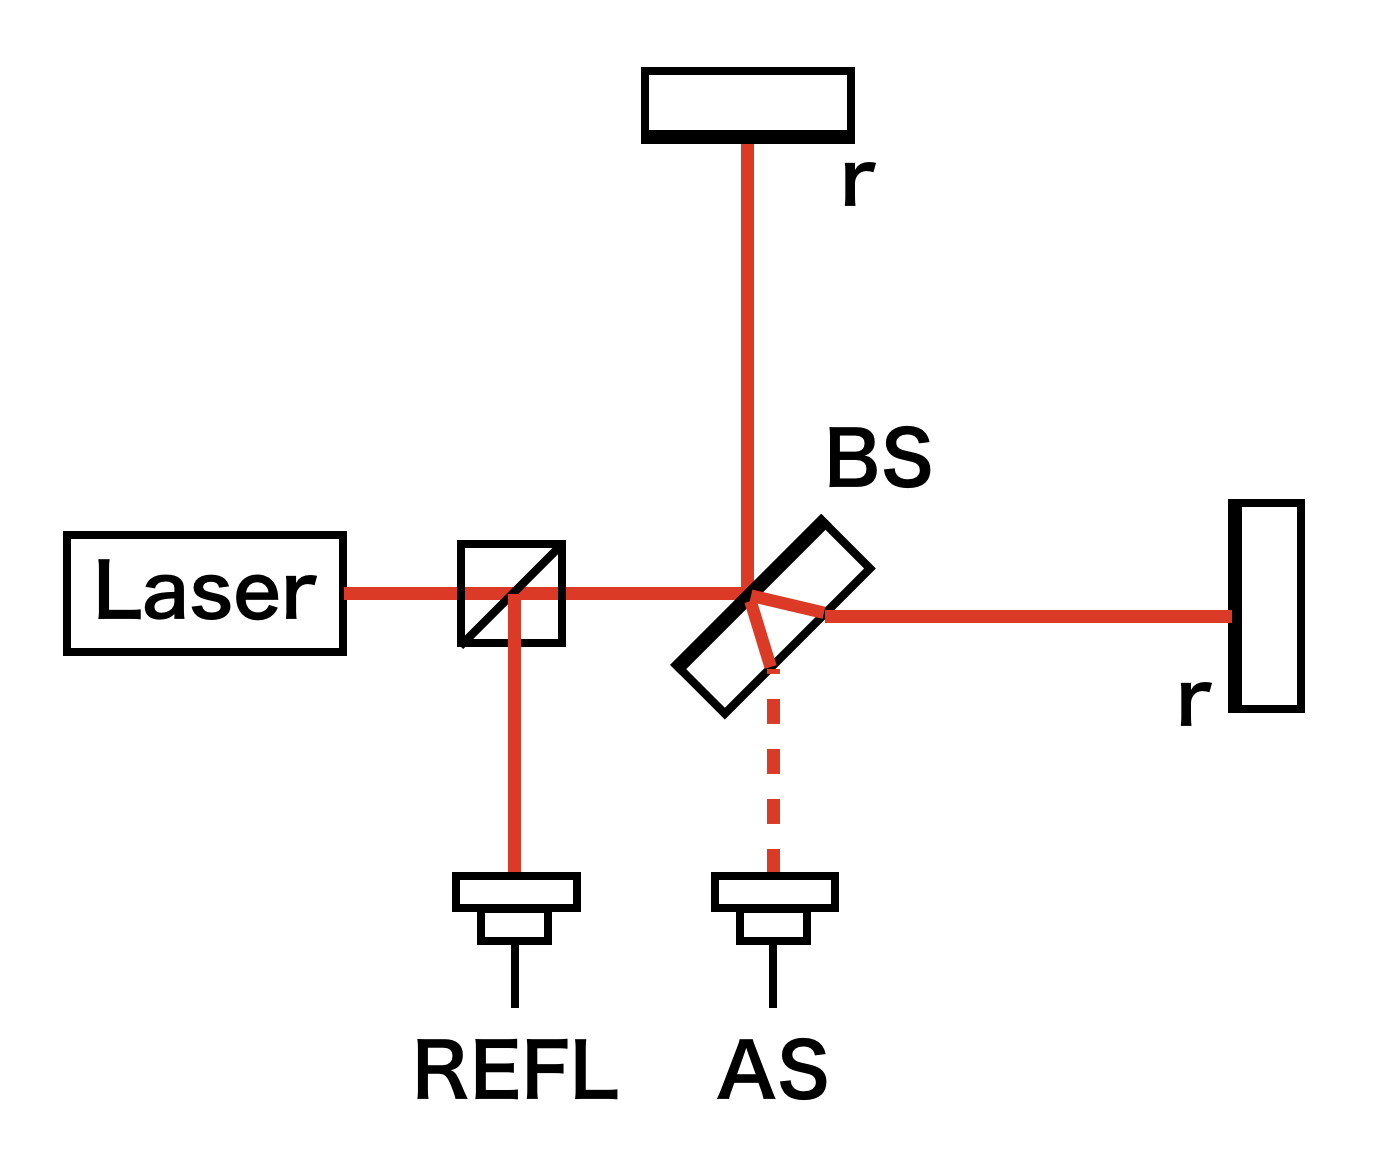
\includegraphics[width=8.0cm]{./img_chap1/img132.png}
    \caption{Michelson Interferometer. }\label{img:img132}
  \end{center}
\end{figure}

Michelson interferometer converts from the differential optical phase of two lights, which propagate each arm, to the amplitude modulation of single output light. Consider about the interferometer shown in Figure  \ref{img:img132}. Incident light is given as,
\begin{eqnarray}
  E_{\mathrm{in}} = E_{0} e^{i\omega{t}},
\end{eqnarray}
where $E_0$ is the amplitude, and $\omega_0$ is the angular frequency of the laser field. 
Two lights split by the Beam Splitter (BS) interfere at the Anti-symmetric (AS) port and Reflection (REFL) port. One can represent the output field at the AS port  as,
\begin{eqnarray}
  E_{\mathrm{AS}} = -\frac{1}{2}rE_{0} e^{i\left(\omega_{0} t-\phi_{x}\right)}+\frac{1}{2}r E_{0} e^{i\left(\omega_{0} t-\phi_{y}\right)},
\end{eqnarray}
where $r$ denote the amplitude reflectivity of the end mirrors, and $\phi_{x}$ and $\phi_{x}$ are the phase delay due to the light traveling in the $x$ and $y$ arms. This output signal can be represented as a single fieled as,
\begin{eqnarray}
E_{\mathrm{AS}} = i r E_{0} e^{i\left(\omega_{0} t-\left(\phi_{x}+\phi_{y}\right) / 2\right)} \sin \left(\frac{\phi_{x}-\phi_{y}}{2}\right). \label{eq:eq132}
\end{eqnarray} 
We find that the amplitude of the output light is a function of the difference between two phases; $\phi_{x}-\phi_{y}$. Here, the power of output light at the AS port is obtained by squaring the Eq.(\ref{eq:eq132}), 
\begin{eqnarray}
  P_{\mathrm{AS}} &=\left[r\sin({\phi_{-}})\right]^2P_0  \label{eq:eq133}
\end{eqnarray}
Similarly, power of the output light as REFL port is written as,
\begin{eqnarray}
  P_{\mathrm{REFL}} &=\left[(r\cos({\phi_{-}}))\right]^2P_0. \label{eq:eq134}
\end{eqnarray}
%Therefore, we can measure the optical phase difference modulated by GW plus mode as the amplitude changes by using a photo detector (PD).

\subsection{Response to GWs} \label{sec:sec122}
The Michelson interferometer is sensitive to the quadrupolar strain caused by the gravitational waves shown in Figure \ref{img:img131}. For example, when the plus mode of the gravitational-wave incidents perpendicularly to change the length of both arms the most, the difference of the optical phase $\Delta{\phi_{-}}$ on the arms of length $L$ is given by \cite{Adhikari2014}
\begin{eqnarray}
  \Delta{\phi_{-}} \sim 2h_{+}\frac{2\pi{L}}{\lambda}. \label{eq:eq_}
\end{eqnarray}
Thus, the Michelson interferometer can measure the length change of the space-time caused $h_{+}L$ by the gravitational-wave.

Figure \ref{img:img130} shows an interferometer antenna response for gravitational-waves with puls and cross modes. The interferometer locates at the center with the two arms parallel to the $x$ and $y$ axes. The unpolarized waves is a quadrature sum of the two patterns. The averaged pattern shows that the interferometer has a wide directivity, and means the single detector is difficult to determine the direction of the source in the sky.
\begin{figure}[h]
  \begin{center}   
    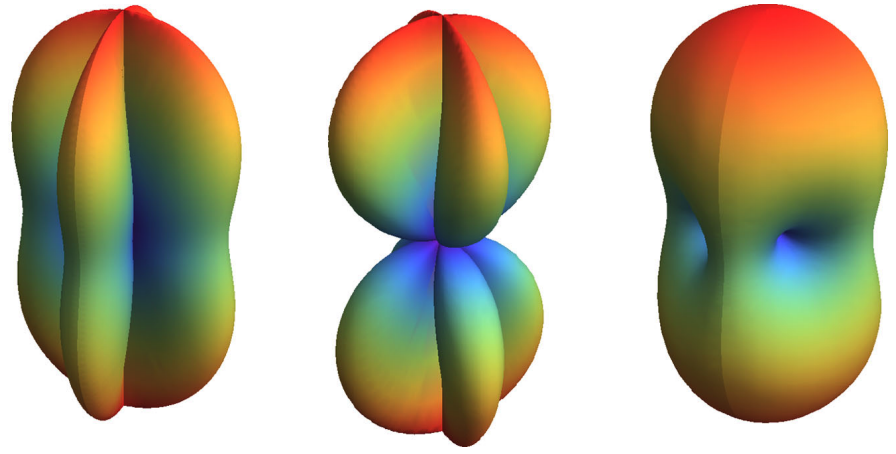
\includegraphics[width=8.0cm]{./img_chap1/img130.png}
    \caption{Antenna patterns of the Michelson interferometer for the plus-mode (left) , the cross-mode (middle), and unpolarized waves (right) \cite{Adhikari2014}. }\label{img:img130}
  \end{center}
\end{figure}

\subsection{Multiple Detection for GW Observation}\label{sec:123}
Gravitational-wave observation generates various physics that cannot be obtained by conventional electromagnetic-wave observation, for which multiple detections are indispensable. The detector does not determine the direction of arrival because of its wide directivity. Therefore, a simultaneous observation by multiple instruments is essential for gravitational-wave astronomy. To verify the theory of gravity in a strong gravitational field, it is necessary to investigate the polarization pattern of gravitational waves, which requires four detectors.             

Depending on the number of units, we can obtain various physics. Although one or two detectors do not determine the direction of the GW sources, if a neutrino detector exists, we can obtain the core state of the supernovae explosion comparing the time difference between the GW and neutrino signals \cite{yokozawa2015probing}. In the case of three detectors, we can determine the direction. For example, in the neutron star merger event, a gravitational wave signal from the event can be detected before other electromagnetic signals, enabling multi-messenger observations. In four detections, we can determine the polarization pattern of the GW \cite{takeda2018polarization}. There are only two polarization patterns in general relativity, but if other polarizations exists, the new polarizations imply the existence of gravity theory beyond general relativity. Furthermore, the four detections also increase the duty cycle in which at least three detectors are operating simultaneously, thereby multi-messenger observation will detect more GWs from compact binary coalescence.


\section{Enhancement of the Sensitivity} \label{sec:13}
\begin{figure}[h]
  \begin{center}   
    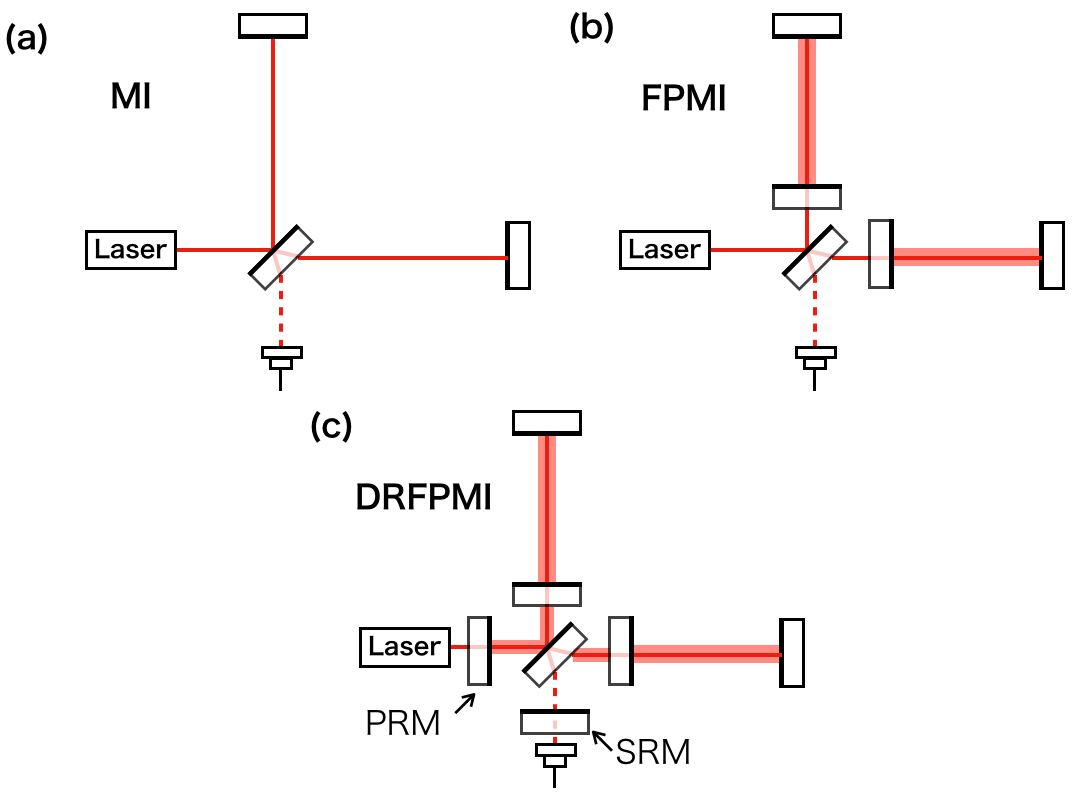
\includegraphics[width=14cm]{./img_chap1/img133.png}
    \caption{Configuration of interferometric GW detector. (a) Michelson interferometer (MI) (b) Michelson interferometer with two Fabry-Perot optical cavities (FPMI). (c) Dual-Recycled FPMI (DRFPMI)} \label{img:img133}
  \end{center}
\end{figure}
In order increase the sensitivity, current interferometric GW detector use the Dual-Recycled Fabry-Perot Michelson Interferometer (DRFPMI). 


\subsection{Fabry-Perot Michelson Interferometer (FPMI)}
According to Eq.(\ref{eq:eq_}), we need the large-scale interferometer. Fabry-Perot optical cavity enhances the effective arm length of the interferometer.

Fabry-Perot optical cavity increase the effective baseline linegth. Consider the Fabry-Perot optical cavity composed of two mirrors separated by L as shown in Figure \ref{img:img133a}. In this figure, $E_{\mathrm{in}},\,E_{\mathrm{r}},\,E_{\mathrm{t}},\,E$ are the incident, reflected, and transmitted fields respectively, $r_{j}$ and $t_{j}$ are the amplitude reflectivity and transsivity of $j$-th mirrors ($j=1,2$). The averaged bounce number in a Fabry-Perot cavity $\mathcal{N}_{\mathrm{FP}}$ is written as \cite{ando1999power}
\begin{eqnarray}
  \mathcal{N}_{\mathrm{FP}} = \frac{2\mathcal{F}}{\pi},
\end{eqnarray}
where $\mathcal{F}$ is a finesse given as
\begin{eqnarray}
  \mathcal{F}=\frac{\pi \sqrt{r_{1} r_{2}}}{1-r_{1} r_{2}}.
\end{eqnarray}

Here, we note that the arm length enhancement can work in case that the cavity length fluctuation is within the linewidth calculated as the full width at half maximum (FWHM);
\begin{eqnarray}
  L_{\mathrm{FWHM}} = \frac{\lambda}{2\mathcal{F}}\label{eq:eq131}.
\end{eqnarray}


\begin{figure}[h]
  \begin{minipage}[b]{0.5\hsize}
    \begin{center}   
      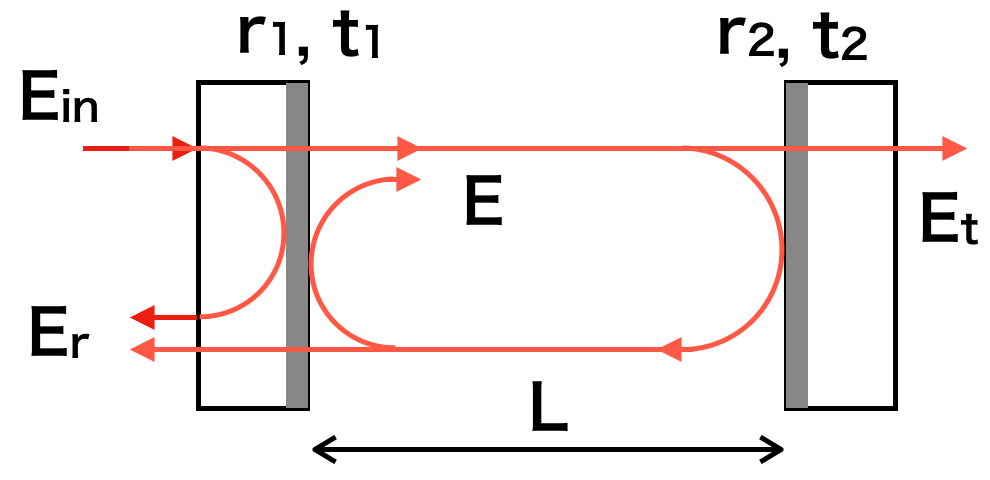
\includegraphics[width=7cm]{./img_chap1/img133a.png}
      \subcaption{Fabry-Perot optical cavity composed of two mirrors separated by L. } \label{img:img133a}
    \end{center}
  \end{minipage}\hspace{3pt}
  \begin{minipage}[b]{0.5\hsize}
    \begin{center}   
      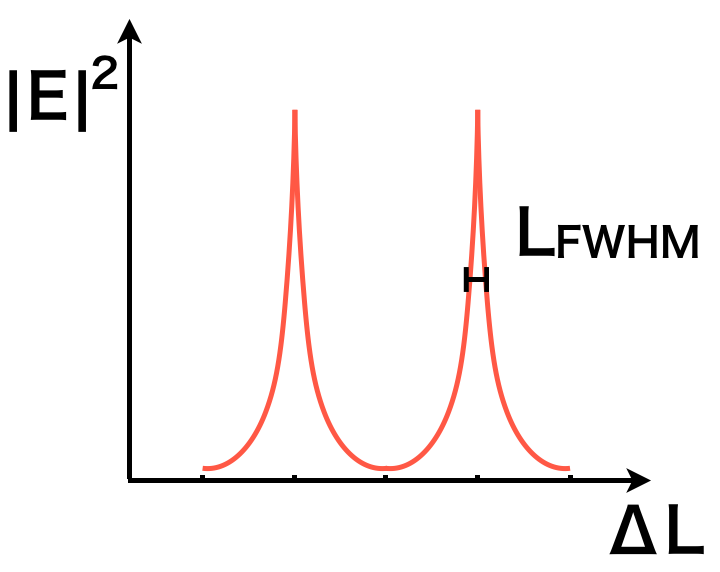
\includegraphics[width=5cm]{./img_chap1/img133b.png}
      \subcaption{Intra-cavity power as a function of displacement of cavity length.} \label{img:img133b}
    \end{center}    
  \end{minipage}
  \caption{Fabry-Perot optical cavity.}
\end{figure}


\subsection{Dual-Recycled FPMI (DRFPMI)}
As shown in Figure \ref{img:img133}(c), the final configuration of the current GW detector is DRFPMI which has two recycling optical cavity \cite{meers1988recycling}.

\subsubsection{Power Recycle}
In order to decrease shot noise, GW detectors use the power recycling technique. In this technique, an additional mirror is installed between the laser and the interferometer to increase the effective laser power by recycling the reflected light from the interferometer. If we increase the laser power, the noise to signal ratio of shot noise decreases as mentioned later.

\subsubsection{Signal Recycle}
The signal recycling mirror installed on the AS port is for tunning the frequency band of the GW signal. This mirror enhances the GW signal by recycling the output signal from the interferometer.

\subsection{Noise}
In terms of the interferometric GW detector, noise can be classified into two noises; detection noise and displacement noise of the test mass. The former noises are the shot noise, the laser power noise, and laser frequency noise.


\subsubsection{Detection noise (Shot Noise)}
In an ideal case that the test mass is not disturbed, which means the mass behaves as the free mass, the shot noise limits the noise of the interferometer.

Shot noise is a noise associated with the fluctuation of the number of photons at the photodetector. In case that the number of photons $N$ is large enough ($N\gg1$), the number of photons obey the Gaussian distribution with the standard deviation of $\sqrt{N}$. Therefore, if laser power $P$ incidents in the detector, shot noise has a relation with the power;
\begin{eqnarray}
  P_{\mathrm{shot}} \propto \sqrt{P}.  \label{eq:eq136}
\end{eqnarray}
One can find that shot noise is a white noise, which propotional to the square-root of the light power $P$.

Here, the relative error of power at the PD is given by 
\begin{eqnarray}
  \frac{\Delta P_{\mathrm{AS}}}{P_{\mathrm{AS}}}  \propto \frac{1}{\sqrt{P_{\mathrm{0}}}},  \label{eq:eq136}
\end{eqnarray}
where $P_{\mathrm{AS}},\,\Delta P_{\mathrm{AS}}$ are the power at the PD, $P_0$ is the power of the incident light. This shows that the increased input laser power can decrease the shot noise. For this reason, we increase the input laser power using power recycling mirror.

\subsubsection{laser frequency fluctuation}
The actual interferometer has an asymmetricity in the arms, which causes the noise coupling from the laser frequency fluctuation. Thus, before inputting the beam to the interferometer, GW detectors use the frequency stabilization system.

\subsubsection{laser power fluctuation}
The laser power fluctuation also contaminates the sensitivity of the GW detectors; thus, the intensity stabilization system (ISS) is used for reducing the noise.

\subsubsection{Seismic Noise}
Seismic noise is the most trouble displacement noise for interferometric GW detectors. Seismic waves from various excitation sources disturb the test mass through the mechanical structures. Therefore, the test masses should be suspended by pendulums to attenuate the seismic noise. 

The pendulum used in GW detectors is a multi-stage pendulum designed to have as low an eigenfrequency as possible. The pendulum acts as a mechanical filter. For example, in the case of a single-stage pendulum with a spring constant of $k$, the frequency transfer function from the ground to the test mass of $M$ can be expressed as
\begin{eqnarray} \label{eq:eq502}
  H(f) \equiv \frac{1}{1-(f/f_0)^2},
\end{eqnarray}
where $f_0 = (k/M)^{1/2}$ is the resonant frequency of the oscillator. According to this equation, the vibration isolation ratio is of the second order above the resonance frequency. When the number of stages becomes N, the vibration isolation ratio becomes 2N. Thus, the multi-stage pendulum can and efficiently reduced the ground vibration. In the case of KAGRA, they use a 9-stage pendulum to obtain a sufficient vibration isolation ratio above 10 Hz.

On the other hand, although a pendulum with a lower resonance frequency is required to expand the band in which the pendulum can attenuate, it is limited to the eigenfrequency of less than 1 Hz. In other words, the passive type seismic isolator cannot attenuate the seismic noise below 1 Hz.  Moreover, the low-frequency seismic noises in this band make the operation of the gravitational wave detector unstable.

\subsubsection{Newtonian noise}
Unlike the seismic noise mentioned above, the Newtonian noise is a noise that the density fluctuation of surrounding objects disturbs the test mass by gravitational interaction \cite{harms2015terrestrial}. Because this noise propagates through space, the seismic isolation cannot isolate the noise. Although the noise does not affect the current 2nd generation GW detectors, it will contaminate the next 3rd generation detectors.

In order to reduce the Newtonian noise, the feedforward control using the seismometer array has been proposed \cite{driggers2015noise}.

\subsubsection{Thermal Noise}
In addition to external disturbances such as the seismic origin noise, the mirror substrate, and surface particles caused by the random thermal motion also generate displacement noise. This thermal noise has been classified into two; mirror thermal noise and mirror coating thermal noise \cite{dan2016study}.

The displacement noise of the mirror thermal noise of the mirror with temperature $T$ is given by 
\begin{eqnarray}
  G_{\mathrm{SB}}(f)=\frac{4 k_{B} T}{\omega} \frac{1-\sigma^{2}}{\sqrt{\pi} E w_{0}} \phi_{\mathrm{sub}}(f),
  \label{eq:eq140}
\end{eqnarray}
where $k_{B}$ is a Boltzmann constant, $\omega$ is the angular frequency, $\sigma,\, E,\, \phi_{\mathrm{sub}}$ are a Poisson's ratio, Young's modulus, and mechanical loss angle of the bulk of the mirror respectively, and $\omega_0$ is a beam radius \cite{levin1998internal, numata2003wide}. One can find that the mirror thermal noise is decreased by lower temperature or increase the beam radius.

The displacement noise of coating thermal noise is given by \cite{numata2003wide,harry2002thermal}
\begin{eqnarray}
  G_{\mathrm{CB}}(f)=G_{\mathrm{SB}}(f)\left(1+\frac{2}{\sqrt{\pi}} \frac{1-2 \sigma}{1-\sigma} \frac{\phi_{\mathrm{coat}}}{\phi_{\mathrm{sub}}} \frac{d}{w_{0}}\right), 
\end{eqnarray}
were $d$,$\phi_{\mathrm{coat}}$ are depth and loss angle of the coating.


%\newpage
\section{Duty Cycle of the Terrestrial GW Detectors} \label{sec:14}
In the gravitational-wave observation, which requires simultaneous detection of multiple gravitational waves, a decrease of the duty cycle of each GW detector reduces that of the entire detector network. As we described in section \cref{sec:123}, the more simultaneous multiple detections, the more physics we can obtain. Thus we need to consider the duty cycle.

The observation of the terrestrial GW detectors is disturbed by seismic motions due to environmental changes. We can classify the none observation state into two states; the lock acquisition state and a state of being unable to do so. In the former state, various methods have been proposed and established in the operation of the detectors to decrease. These methods quickly move the interferometer from an uncontrolled state to a controlled state with low-noise configuration enough to observe. On the other hand, the latter state indicates that the present seismic isolation control is insufficient.

In order to improve the duty cycle, it is necessary to optimize the lock acquisition system and the seismic isolation system. Especially in our study focus on the development of the new seismic isolation system. Before we get into the details of the new system, we first give an overview of the current GW detectors. This section presents an overview of the terrestrial GW detector projects and the duty cycle deteriorated by the seismic motions.


\subsection{Overview of the GW Detector Projects}
There are three generations for GW detectors which are categorized by the difference of the baseline length. These detectors are listed in table \ref{tb:tb101}. The first-generation has a baseline length of several hundred meters, the second-generation has several kilometers, and the third-generation has several tens of kilometers. The current working GW detector is the second generation. The third-generation detectors are under planning, but the concept is the underground interferometer using cryogenic mirrors. These two features, underground and cryogenic, are the same as that of KAGRA. KAGRA is the first large-scale cryogenic interferometer constructing in the underground in the GW detector projects, so this detector is also called 2.5 generation GW detector.

\begin{table}[h] 
  \begin{center}
    \caption{Terrestrial laser interferometers \cite{chen2017brief,beker2013low}}\label{tb:tb101}
    \begin{tabular}{llll} 
      \hline
      generation &project & baseline [m] & geological feature \\ \hline \hline
      1st &LISM  & 20    & Granite/gneiss \\ 
      &CLIO  & 100   & Granite/gneiss \\
      &TAMA  & 300   & Sedimentary soil \cite{1970449}\\ 
      &GEO   & 600   & Sedimentary rock \\ \hline
      2nd &aLIGO L1 & 4000  & Sedimentary soil \\
      &aLIGO H1 & 4000  & Sedimentary rock \\
      &aVirgo   & 3000  & Sedimentary rock \\
      &KAGRA   & 3000  & Granite/gneiss \\ \hline
      3rd &ET      & 10000 & (Planning) \\
          &CE      & 40000 & (Under the discussion) \\
      \hline
    \end{tabular}
  \end{center}
\end{table}


\subsubsection{1st Generation}
The first-generation GW detectors (LISM \cite{sato2004ultrastable}, CLIO \cite{ohashi2003design}, TAMA \cite{ando2001stable}, GEO \cite{grote2010geo}) are small-scale interferometer. Although these detectors have performed scientific operations since 1999, no gravitational wave have detected. The operation was the demonstration of the working principle of the key technology to increase the sensitivity, and these detectors have constrained the upper limits to several gravitational wave sources \cite{takahashi2004coincidence, Fairhurst2011}.

\subsubsection{2nd Generation}
The second-generation GW detectors (KAGRA\cite{akutsu2017construction}, Advanced Virgo\cite{acernese2014advanced}, Advanced LIGO\cite{aasi2015advanced}) are the kilo-meter scale interferometers for the enough sensitivity to detect GW signal. The detectors have accomplished not only the first GW detection but also the determination of the direction of arrival,  thereby the multi-messenger astronomy was established. As shown in Figure \ref{img:img192}, the detectors are planning to enhance the sensitivity to reach the design sensitivity of each detector over several years \cite{abbott2018prospects}.
\begin{figure}[h]
  \begin{center}   
    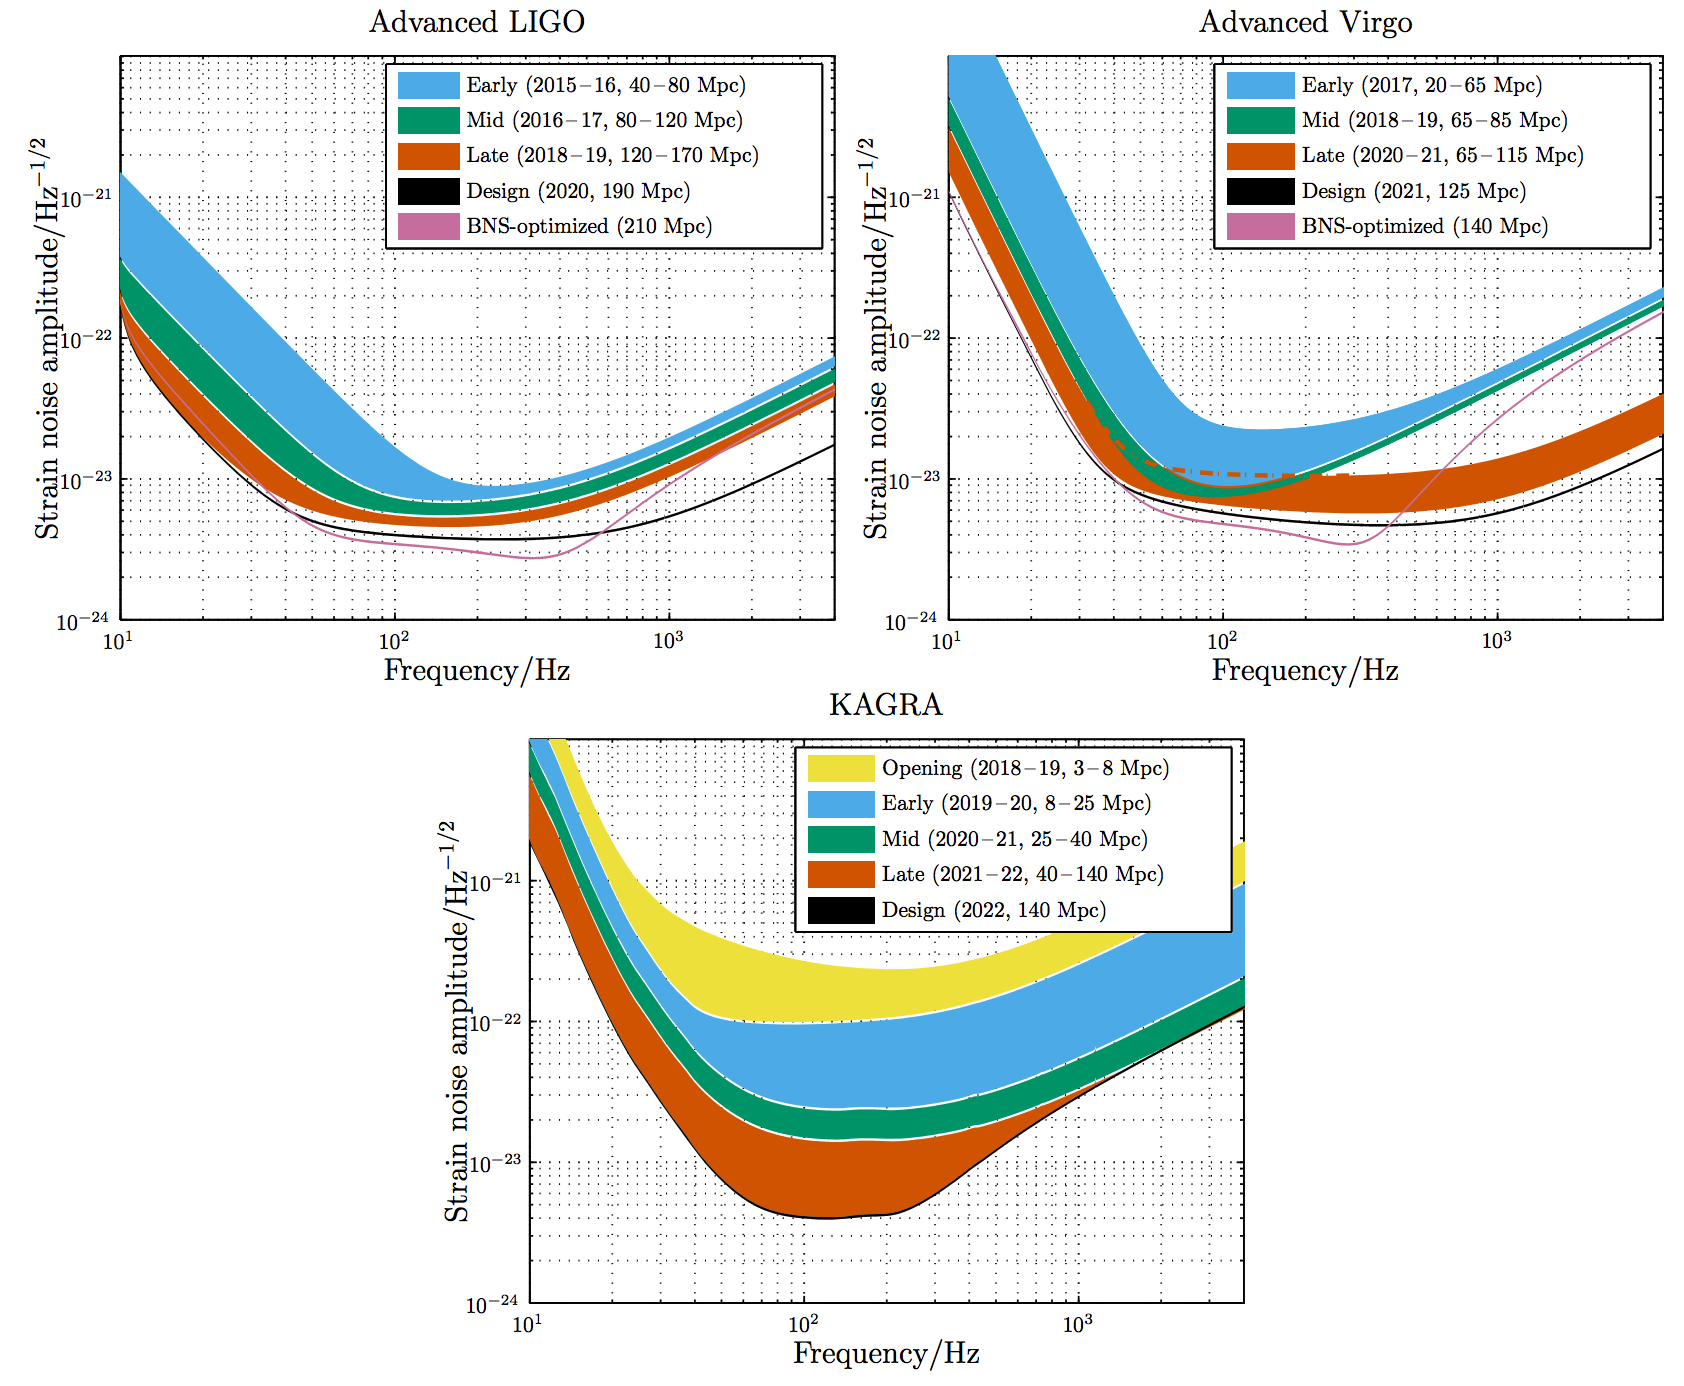
\includegraphics[width=14cm]{./img_chap1/img192.png}
    \caption{Target strain sesitivies of the second-generation detectors \cite{abbott2018prospects}} \label{img:img192}
  \end{center}
\end{figure}


\subsubsection{3rd Generation}
The third-generation GW detector has a ten-kilometer scale interferometers. Einstein Telescope (ET) and cosmic explorer (CE) \cite{abbott2017exploring} are proposed. It aims to reach a sensitivity about a factor of 10 or more better than the second-generation detectors.

The key features of the third-generation detector are the underground and cryogenic mirrors. These features are also the same as that of KAGRA.

\subsubsection{KAGRA}
KAGRA is a first large-scale cryogenic interferometer constructing in the underground. The key features of KAGRA were demonstrated in the first-generation detectors; LISM and LISO. 

LISM, Laser Interferometer GW Small observatory in a Mine, is a first GW detector in the underground to demonstrate the stable performance of the detector. The detector of LISM is the Michelson interferometer whose arms contain $20\,\mathrm{m}$ Fabry-Perot optical cavities. This arm cavity has a high finesse of 25000. Despite such high finesse, the duty cycle was $99.8\,\%$. Such a stable operation is owing to the reduction of the baseline length fluctuation of the bedrock. This reduction effect was confirmed on the sensitivity plot of LISM, as shown in Figure \ref{img:img122}. In this figure, one can find that the sensitivity of the interferometer is less than the noise projection of the horizontal seismic noise below $6\,\mathrm{Hz}$. In this band, the seismic motion moved the baseline as a single object, which means the less baseline length changes. So, LISM could perform a stable operation. 

\begin{figure}[h]
  \begin{center}   
    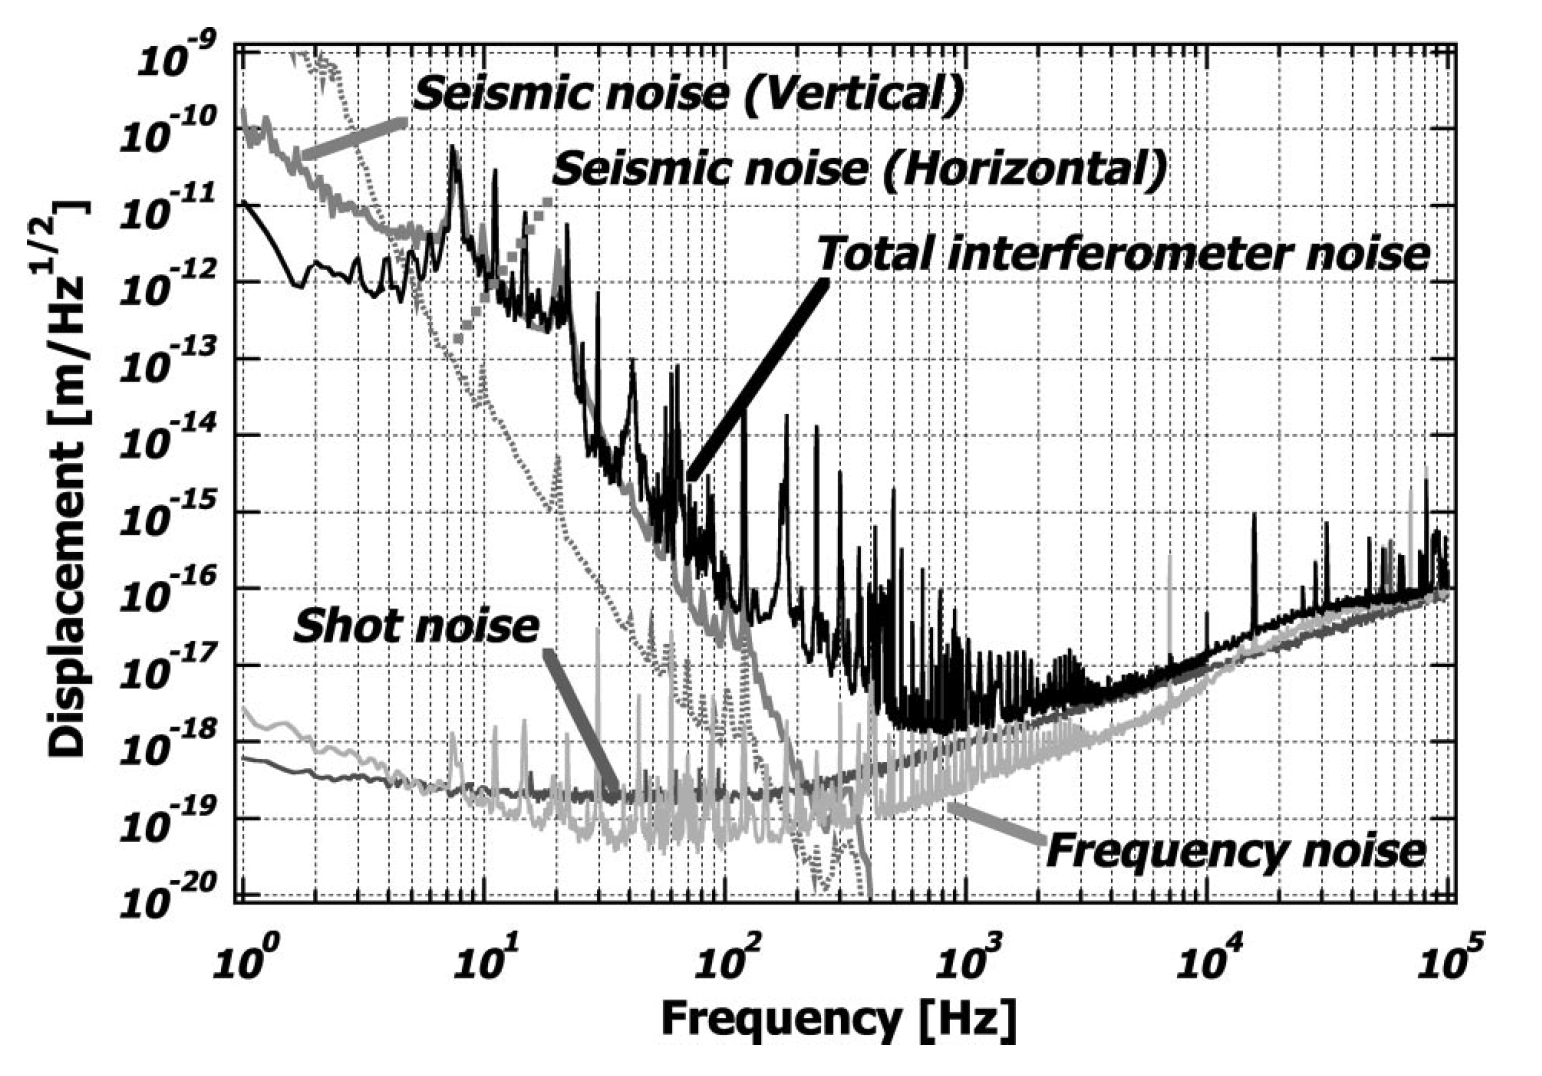
\includegraphics[width=11cm]{./img_chap1/img122.png}
    \caption{The noise equivalent detector sensitivity of LISM \cite{sato2004ultrastable}. } \label{img:img122}
  \end{center}
\end{figure}


CLIO, cryogenic laser interferometer observatory, is an interferometer to demonstrate the thermal noise reduction using sapphire mirrors \cite{ohashi2003design}. In order to confirm the reduction, CLIO is also constructed in the underground to attenuate the seismic noise. Moreover, low-vibration pulse tube cryocooler has developed \cite{tomaru2004development}. Owing to these quiet environment, they demonstrated to reduce the sensitivity limited by the thermal noise using a cryogenic test masses \cite{uchiyama2012reduction}.


\subsection{Duty Cycle} \label{sec:duty}
The duty cycle is the observable time of the telescope. For example, in the case of electromagnetic observation, the observation depends on the atmosphere in the bad weather. Even when the weather does not matter, in the case of the radio telescopes, the field of vision is limited, so we, of course, cannot see objects on the other side of the earth. On the other hand, GW observation is highly permeable and can detect in any direction, even underground. However, since the GW detector has a narrow sensor range while having high sensitivity, the sensitivity depends on the condition of the seismic activity. For example, the interferometer status of LIGO detectors during the first observation (O1) is shown in Figure \ref{img:img190}. The duty cycle of both detectors is about 60\%, and the remaining 40\% caused by two major unobservable states except for other states including maintenance and commissioning. One is the Locking state, which is a transition state from an uncontrolled state to a low-noise configuration. The other is a state of uncontrolled due to environmental changes such as earthquakes, microseismic noise, and so on.

\begin{figure}[h]
  \begin{center}
    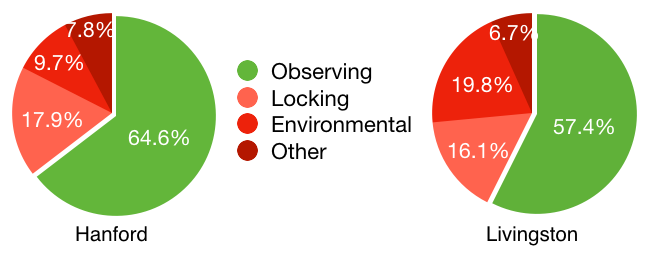
\includegraphics[width=11.0cm]{./img_chap1/img190.png}
    \caption{Interferometer status of LIGO in O1 \cite{abbott2018prospects}. Duty cycle is the observing state. Locking state is the transit state from an uncontrolled state to the lowest noise configuration. Environmental state is the uncontrolled state due to environmental changes. Other includes the planned maintainance and commissioning.}\label{img:img190}
  \end{center}
\end{figure}


\subsubsection{Problematic seismic noises for duty cycle}
Seismic noise below approximately 1 Hz is the cause of the deterioration of the duty cycle because the pendulum used in the GW detector is difficult to attenuate insufficiently. In this frequency band, particularly problematic seismic noises include microseismic noise (0.1 - 1 Hz), long-period earthquakes (0.01 - 0.1 Hz), and earth tides ($10^{-5}$ Hz). For example, during the test operation of KAGRA, there was a correlation between the root mean square amplitude of the ground motion and the duty cycle \cite{akutsu2019first}. In the case of LIGO, owing to an active seismic isolation system using seismometers, the duty cycle is not limited mainly by microseismic noise but limited the long-period earthquakes \cite{Biscans2018control}. This degradation occurs because the sensitivity of the seismometers used for the isolation system is insufficient in the earthquake band.

Furthermore, earth tides cause the saturation of control signals of all GW detectors. Insufficient actuator range causes the degradation of the duty cycle due to the low-frequency seismic noise. In principle, it is desirable to use an actuator that is sufficiently strong and has a broad actuator range for controlling the test mass, but this is not the case in practice. The GW detectors should use a weak actuator so that control noise does not contaminate the sensitivity. 

The influence of low-frequency seismic noise becomes significant in long-scale interferometers. In the case of the short-scale baseline, the low-frequency seismic noise did not disturb the baseline length because the motion moves the arm cavity as a single object. However, in case the long-scale baseline, the seismic motion below $1\,\mathrm{Hz}$ moves the two mirrors of the arm cavity with no correlation. Especially around $0.2\,\mathrm{Hz}$, the amplitude of microseisms caused by ocean activities exceeds the linewidth of the arm cavity. Thus, the low-frequencies seismic noises directly limit the duty cycle of interferometric GW detectors.

Therefore, the low-frequency seismic noise below 1 Hz is a significant problem that decreases the duty cycle. This is an unavoidable problem for the GW detectors aiming for the more lengthened baseline.

\subsubsection{Improvement of duty cycle}
The way to increase the duty cycle is to reduce the locking time and to improve the vibration isolation performance in the low-frequency band.

Arm length stabilization (ALS) is the technique to reduce the locking time. This technique reduces the RMS of arm cavity length using frequency-doubled auxiliary lasers before locking the cavity using the main infrared laser \cite{mullavey2012arm,izumi2012multi}. The wavelength of this auxiliary laser is half of the main infrared laser. Since the linewidth is also half according to Eq.(\ref{eq:eq131}), the auxiliary laser is more comfortable to lock the arm cavity than the main laser. Once locking the arm cavity using the auxiliary laser, the ALS system can reduce the RMS of arm cavity length fluctuation using the feedback signal of the auxiliary system so that the main laser can lock the arm cavity. Owing to this system, lock acquisition end within about 10 minutes.

Although the ALS system can bring the interferometer to the observation state in a sufficiently short time, we cannot use the system in the observation phase due to the high control noise. In the observation state, we can only use the main laser with narrow linewidth as a sensor for measuring the baseline length. Moreover, we have to use a narrow dynamic range and weak actuator not to contaminate the GW sensitivity with the actuator noise. In this situation, if the seismic disturbances exceed the range of the sensors and the actuators, the cavity can not keep the locking state.

An active seismic isolation system has been developed to reduce the RMS amplitude of the arm cavity length during the observing state.  This active system is used to isolate low-frequency seismic noise that is not attenuated in passive pendulum systems, which is described in chapter 4. However, the current active vibration isolation systems are capable of vibration isolation only up to microseismic noise due to the insufficient sensitivity band of the inertial sensor used for control.

In LIGO, the duty cycle is diminished due to an earthquake shaking the ground in the lower band. When the interferometer lost the locking by an earthquake, it takes several hours to return to the observing state. In order to prevent the lock loss, the LIGO detector switches the control filter just before the earthquake hits the site \cite{Biscans2018control}. Although this control filter introduces control noise above the microseismic band, this reduces the enhancement of the RMS amplitude in the earthquake band. The control filter is optimized to improve the duty cycle when earthquakes come.

\section{Outline of thesis} \label{sec:15}
The goal of this study is to improve the duty cycle of GW detectors by isolating the low-frequency seismic noises. We have developed a vibration isolation system for seismic noises. In this thesis, two main topics are described. One is a study of the influence of the low-frequency seismic noise to the large-scale GW detectors. This study shows that the baseline fluctuation is somehow reduced due to a correlated motion at two separate points, and this correlation decrease in the large-scale baseline. For this reason, large-scale GW detectors are suffering from seismic noise. This problem is happening even in the underground. Another topic is the development of the baseline compensation system to reduce residual motion. The feature of this new system is the feedforward control using a strainmeter installed in parallel to the KAGRA baseline, which is named geophysics interferometer (GIF). GIF has been developed for monitoring the deformation of the baseline directly with high sensitivity. The new system compensates for the baseline fluctuation of the arm cavity by using the GIF strainmeter signal.

In \cref{chap2}, we describe the properties of the seismic noise. The GIF strainmeter's working principle and design are described in \cref{chap3}. After that, we describe the baseline compensation system comparing with the current system in \cref{chap4}. In \cref{chap5}, the demonstration of this new system implemented on the KAGRA X-arm cavity, and the result is described. At the end of the thesis, \cref{chap6}, we describe a conclusion and future directions.

%% \section{Summary of the Chapter}
%% GWs are ripples in space-time and are caused by the motion of the massive object in the universe. The observation of gravitational waves not only reveals the structure of space-time but also provides us various information about high-energy astrophysical phenomena.

%% The GW detector is a Michelson interferometer type laser interferometer with an optical resonator. At present, four second-generation interferometers are constructed on the earth to observe GWs.

%% Improvement of stability of GW detectors is important in GW observation which needs multiple simultaneous detections. The duty cycle is limited mainly by low-frequency seismic noise. Thus a vibration isolation system is required to prevent the instability of operation.
